\documentclass{article}
\usepackage{geometry}
\usepackage[document]{ragged2e}
\usepackage{csquotes}
\usepackage{hyperref}
\usepackage{graphicx}
\geometry{a4paper,total={170mm,257mm},left=20mm,top=20mm}
\newcommand\independent{\protect\mathpalette{\protect\independenT}{\perp}}
\def\independenT#1#2{\mathrel{\rlap{$#1#2$}\mkern2mu{#1#2}}}
\begin{document}
    \begin{titlepage}
        \begin{center}
            \vspace*{1cm}
            
            \textbf{Probabilistic Models Project Proposal}
            
            \vspace{0.5cm}
            
            
            \vspace{1.5cm}
            
            \vfill
            
            Final Project\\
            
            \vspace{0.8cm}
            
            
            
            Computer Science\\
            IDC\\
            \today
            
        \end{center}
    \end{titlepage}
    \textbf{Intro}\\
    Probabilistic Graphical Models (PGM) use a graph representation to describe complex distribution over high dimensional space. Where Every node in the graph correspond a random variable, and edges in the graph correspond to direct probabilistic interactions between variables. This representation is a set of in-dependencies holds in the distribution.\\
    In high dimensional distribution the graph representation encode the probability in small factors rather then over every possible assignment of the variables, and the joined distribution defined as the a product of all these factors. In this kind of representation we can define Bayesian network and Markov network distributions in a visual way. Where the Bayesian network is represented as a directed graph and Markov as undirected graph.\\
    This representation allow humans to better evaluate properties and semantics of a variables distribution, it can help understand unexplained or undesirable answers. In addition using the graph to analyses data, it is possible to run efficient algorithm to posterior probability of variables given the evidence of others. Another characteristic is learning from data model provides a good approximation of past experience.\\~\\

    The main objective of this project is to develop a user-friendly software tool for constructing PGMs and experimenting with different aspects and inference algorithms. This tool will be designed both for educational use in academic courses and for self exploration by scientists and developers in the industry. This tool illustrates different aspects of probabilistic models in 6 different units:
    \begin{enumerate}
        \item Unit 1 - conditional independence in Bayesian networks. Random variable independence through PGM, including conditional independence using D separation.
        \item Unit 2 - undirected representations of Bayesian networks. Different representation of PGMs
        \item Unit 3 - elimination orders. Learn how to calculate joint probability for some nodes in Bayesian network, and marginal probability for some set of variables in the network
        \item Unit 4 - inference algorithms
                Inference of observed random variables by a set of inferred random variable
        \item Unit 5 - parameter inference
        \item Unit 6 - sampling algorithms on general Probabilistic Graphical Models
    \end{enumerate}
    A more comprehensive explanation on every unit can be found in proposed design section. The tool designed to experiment basic understanding from dependencies of random variables, until running different algorithms on Bayesian networks.\\~\\

    In our research we came across a couple of libraries implements different algorithms on PGMs. Although those libraries have some aspects in common with our tool, we believe our tool helps to experiment in PGMs more gradually. Most of the libraries offer an efficient code, sometimes with visual representation, but not for learning purposes. Here is the list of tools:
    \begin{enumerate}
        \item Kevin Murphy - THe most comprehensive tool we found, an assemble of Matlab libraries implements various probabilistic models. Most of the libraries written by Kevin Murphy along with his students. Some of the libraries are:
            \begin{enumerate}
                \item PMTK - A collection of Matlab functions, written to support Kevin Murphy textbook ``Machine learning: a probabilistic perspective''.
                \item DAG structure learning using L1 regularization - A library to find Markov blankets using L1
                \item Bayesian DAG learning - Bayesian inference over DAG (directed acyclic graph). This library cannot handle undirected graphs and inference with hidden nodes.
            \end{enumerate}
        \item Hidden Markov Model Toolbox - Written By Kevin Murphy in 1998, support inference for HMMs (Hidden Markov Model), implemented on Matlab
        \item OpenGM - A C++ Implementation for discrete factor graph models. The main objective of this library is to give efficient implementation, and not a learning experience.
        \item Probabilistic Graphical Models - A Matlab implementation for inference and learning Bayesian and Markov networks hosted on Github. The library gives a code to learn PGM, but lack the visualization part.
    \end{enumerate}

    \pagebreak

    \textbf{Proposed Design}\\
    As stated in the introduction the tool is build from 6 units, in this section we are going to elaborate on each one. Every unit extends the capabilities of the former unit.ֿֿ\\
    Before we dive into every unit, let us define the basic capability this tool, give the user the ability to define a Bayesian network in two basic steps:
    \begin{enumerate}
        \item Define all nodes of the network that represent random variables
        \item For every node the user is able to define it's parents. Where a node can have 0 or more parents
    \end{enumerate}
    This way the user is able to visual his network as a directed graph and explore it.
    \begin{enumerate}
        \item Unit 1\\
        This unit is the designed to learn the basics of probabilistic models through a visual representation of Bayesian network, as a directed graph without the probability definition of every node.
        \begin{enumerate}
            \item Explore conditional independence, using D separation criteriation. The D separation is a general criterion for deciding from a given graph whether a set of variables X are independent of another set U given another set A. Or more formally: $X_V \independent X_U | X_A$.\\
            The user is going to be able to choose two nodes to check independence for, and a set of nodes to condition on, all on the graph representation of Bayesian network. The tool is going to show if those nodes are independent. Highlight on the graph the paths that block dependency
        \end{enumerate}

        \vspace{0.5cm}

        \item Unit 2\\
        This unit objective is understanding the undirected graph representation of the Bayesian network. In the unit we are still not taking the probability of the nodes into consideration for all operations. 
        \begin{enumerate}
            \item 
             In one click the user can convert the directed graph representation to an undirected graph, called the moralized graph. In this undirected representation parents of a node in the original graph will have a new edge between them. This emphasize the fact that all variables in the same conditional probability form a clique.
            \item Validate if graph is chordal or not. The main characteristic of this graph is that every cycle of four or more vertices have a chord, in other words every included cycle in the graph should have exactly three vertices. This representation can help the user understand if perfect elimination exists or not in the for the next unit.
            \item Convert moralized graph to factor graph. A bipartite graph representation with one class representing nodes in original graph and the other class representing maximal cliques.
        \end{enumerate}
        \item Unit 3\\
            The main objective of this unit is to show calculation of joint and marginal probability of nodes in the graph representation . This unit does not show the actual calculation, but focus on implication of elimination. Still this unit refer to graph representation without referring to the probability table of every node.
        \begin{enumerate}
            \item Show elimination algorithm implementation on graphs. User can run elimination algorithm step by step. On every step the user choose a node to eliminate, on the graph the user can see the new edges added to the graph.
            \item Try to find a prefect elimination order, choose one simplical node and start elimination from there, write the order on the screen, on every step find the next simplical node, if there is not such one, the user will be able to choose the next node to eliminate.
        \end{enumerate}
        \item Unit 4\\
            In this unit the main objective is to show calculation of joint and marginal probability of random variables. The difference in the unit is here the probability tables are part of the calculation.
            Show message passing algorithm in graph representation. The user can have the ability to run the algorithm to calculate:
            \begin{enumerate}
                \item Marginal distribution - calculates marginal distribution for every node
                \item Max probability assignment - computes assignment of unobserved nodes with observed nodes 
            \end{enumerate}
            In addition the user has the ability to run in two execution modes: 
            \begin{enumerate}
                \item Full run, in this mode the algorithm runs and calculates marginal distribution for all nodes in the background. When the results are ready, the user is able to see marginal for a node by selecting that node
                \item Step by step, on every step show marginal calculated for the node starting in root. This only applies to distribute step of the algorithm, still the collect part of the algorithm runs in single step.
            \end{enumerate}
        \item Unit 5 \\
            Parameter inference through data in tree models
        \item Unit 6\\
        \begin{enumerate}
            \item Markov chain Monte Carlo algorithm
        \end{enumerate}
    \end{enumerate}

    \textbf{Implementation Demo}
    \begin{figure}[h!]
        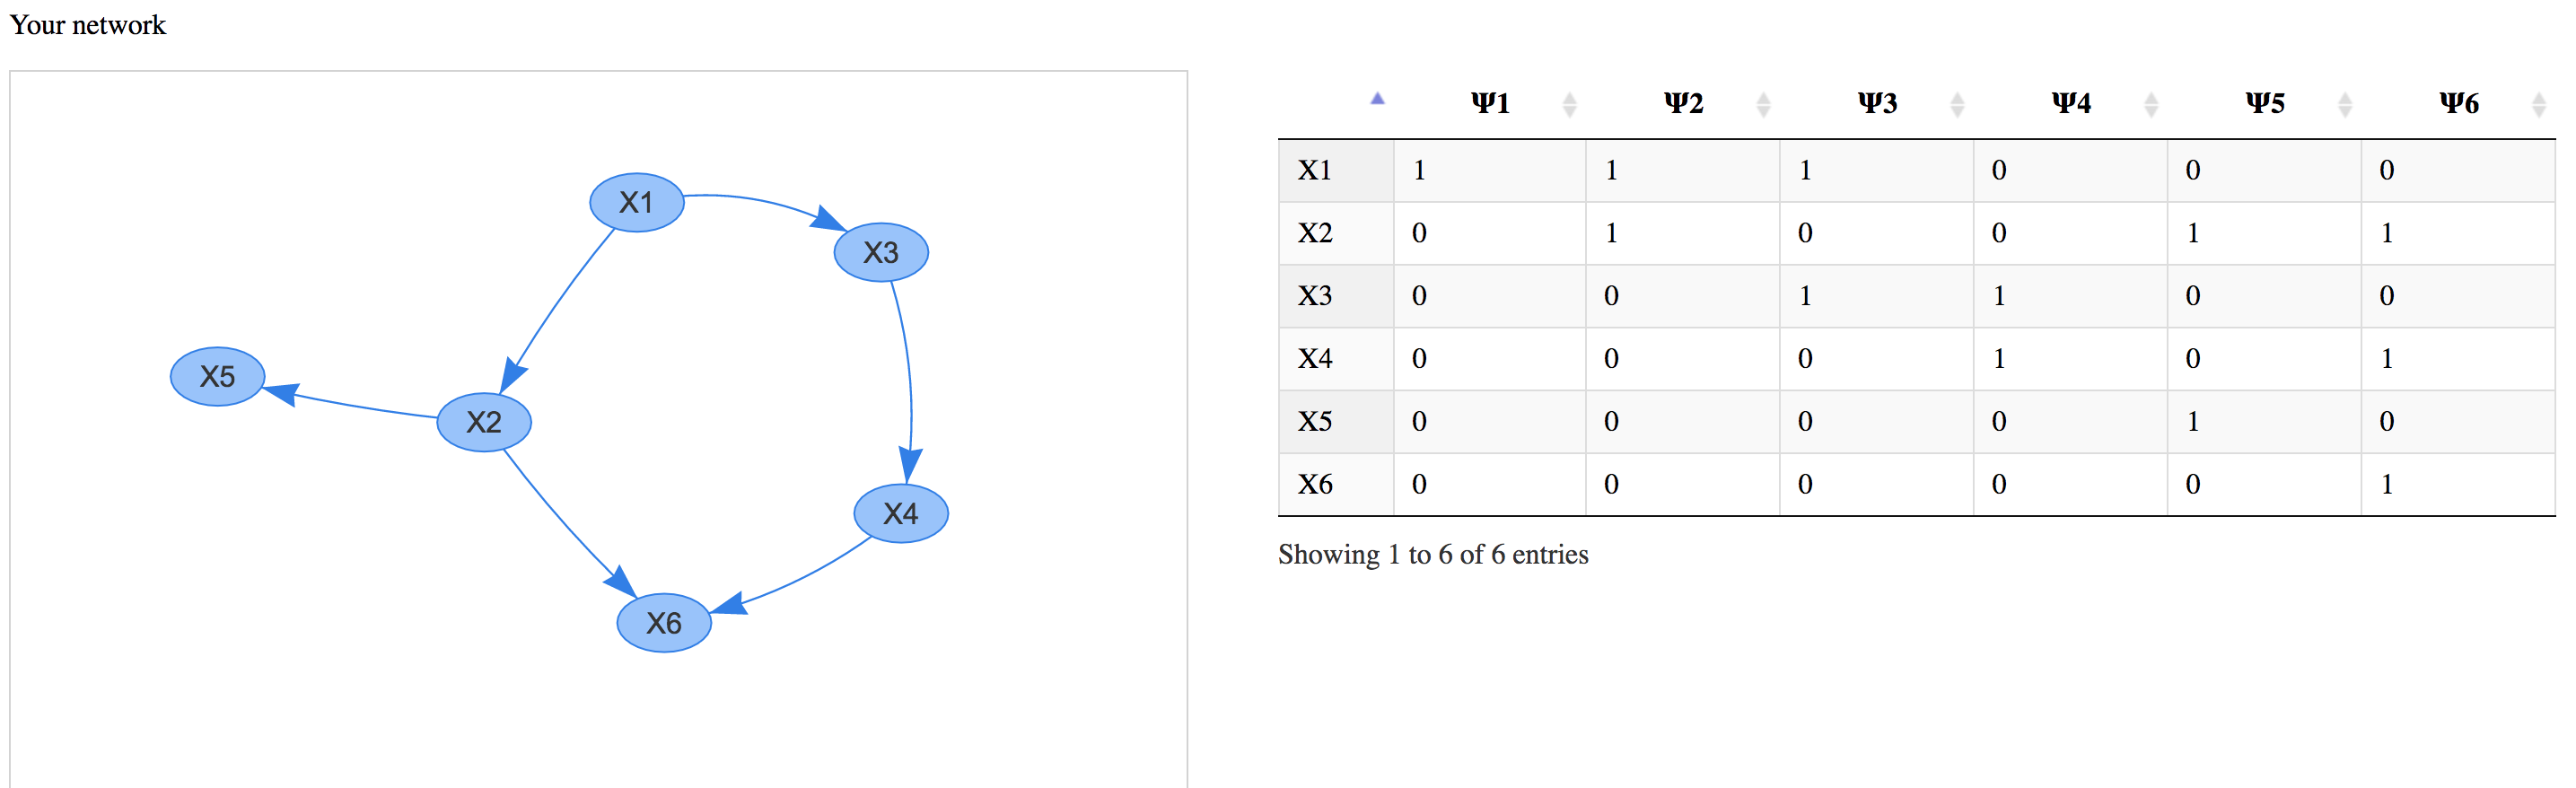
\includegraphics[width=\linewidth]{img/network_binary_matrix.png}
        \caption{Bayesian network representation by DAG with binary membership table.}
        \label{fig:besian_network}
    \end{figure}

    \begin{figure}[h!]
        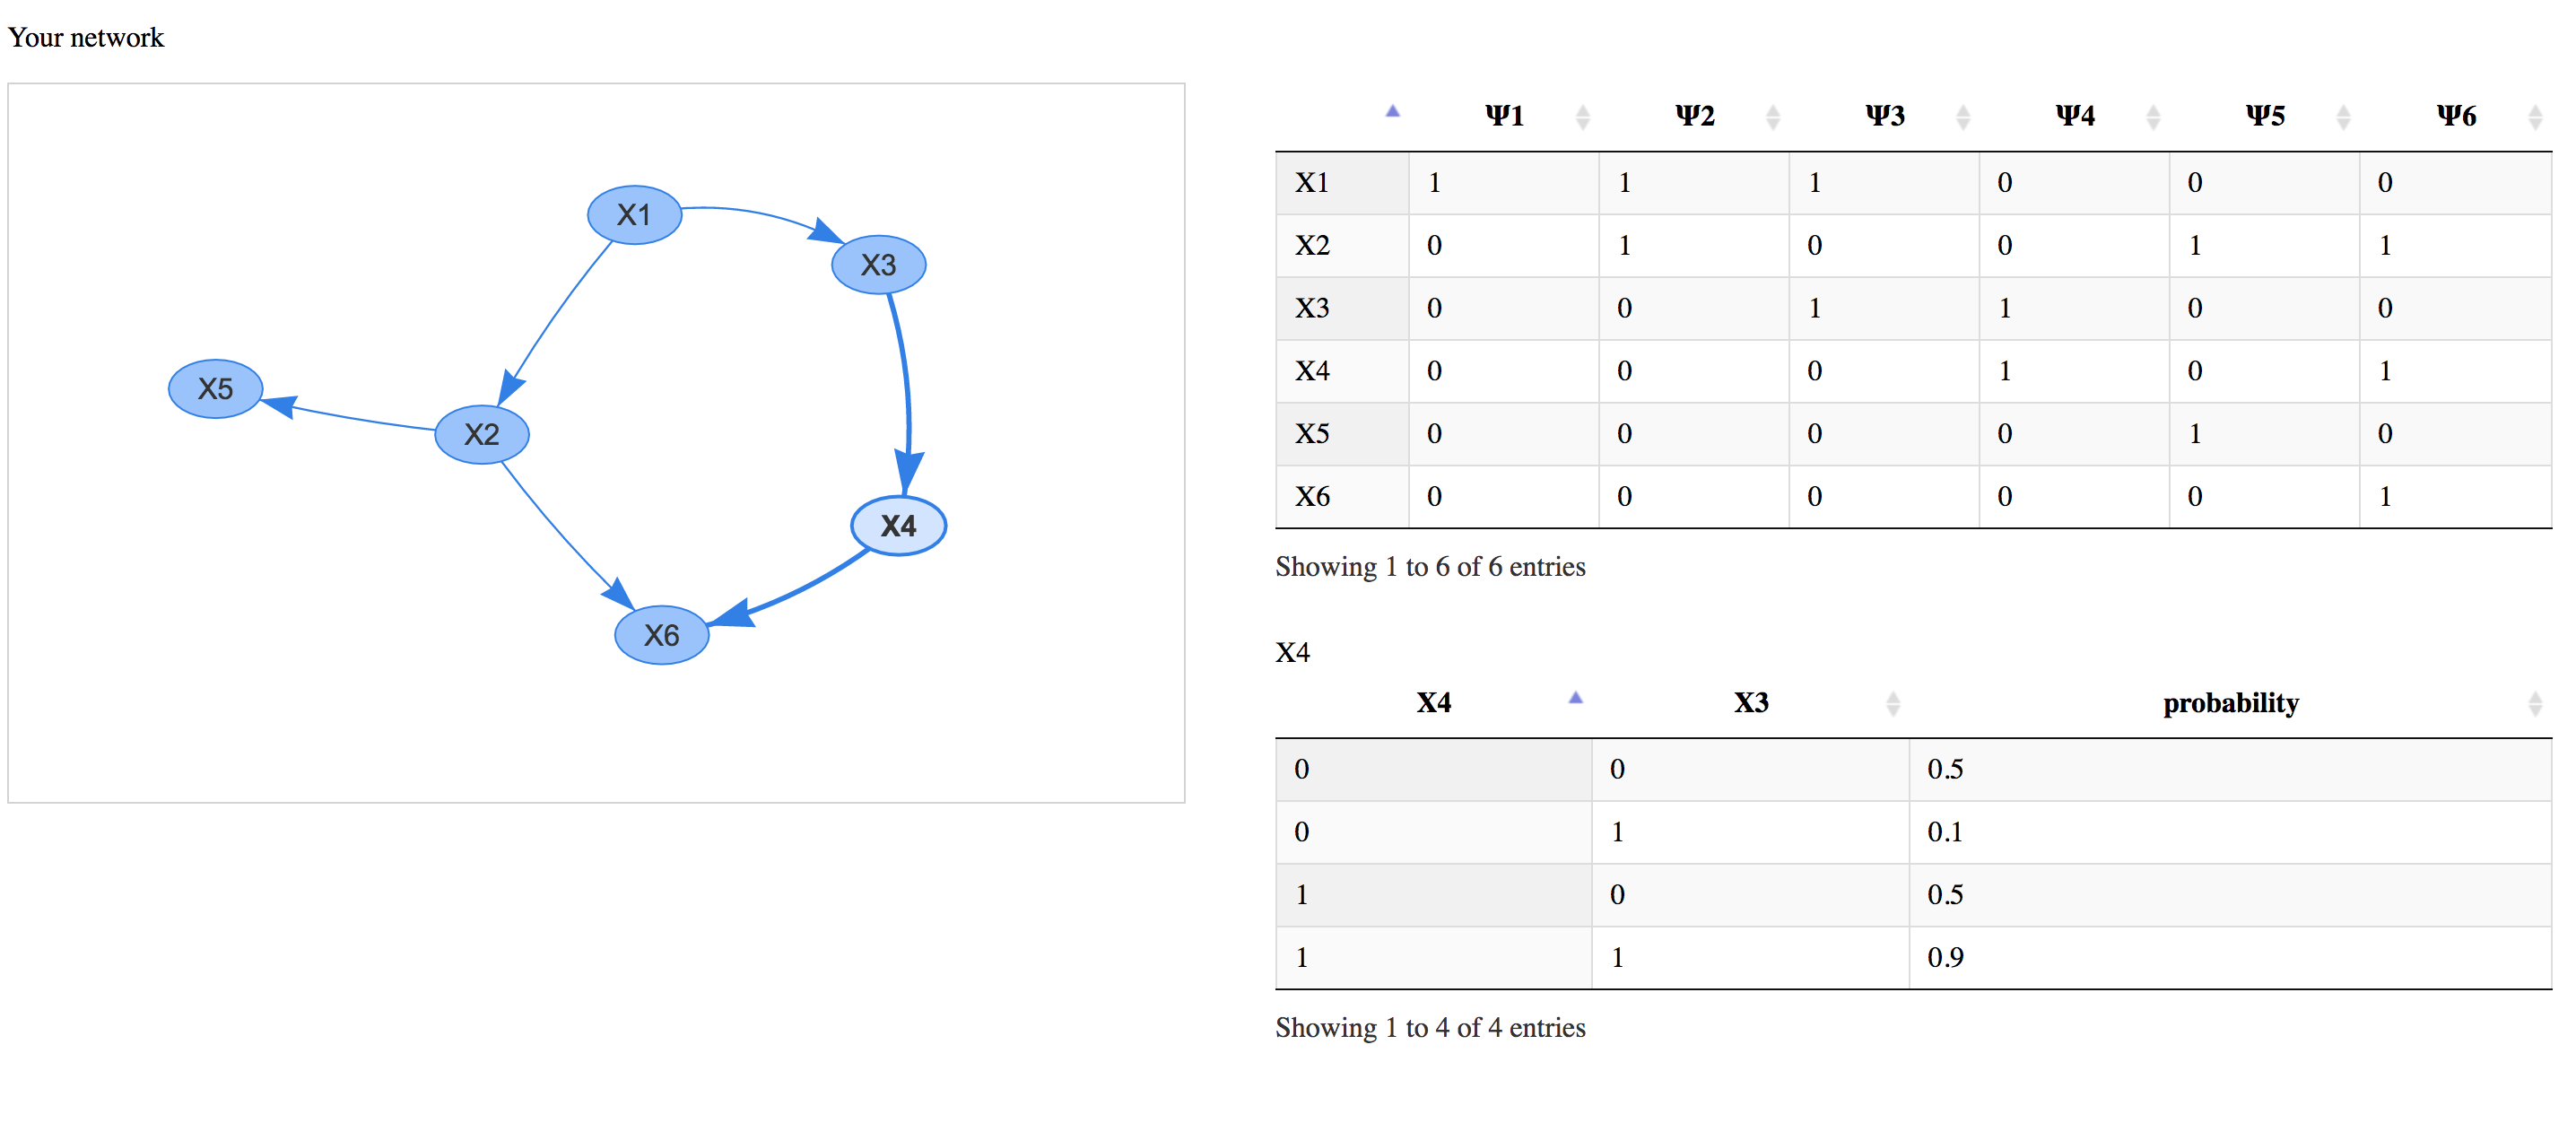
\includegraphics[width=\linewidth]{img/network_selected_node_table.png}
        \caption{Bayesian network representation by DAG, after one node is chosen, show it's potential function table.}
        \label{fig:besian_network_chosen_node}
    \end{figure}

    \vspace{0.5cm}
    \begin{thebibliography}{9}
        \bibitem{Kevin Murphy}
        Kevin Murphy and students libraries \\\texttt{http://www.cs.ubc.ca/\~{}murphyk/Software/}
        \bibitem{Hidden Markov Model Toolbox}
        Kevin Murphy toolbox for inference on Hidden Markov Models \\\texttt{http://www.cs.ubc.ca/\~{}murphyk/Software/HMM/hmm.html}
        \bibitem{OpenGM}
        OpenGM C++ library for discrete graph models \\\texttt{http://hciweb2.iwr.uni-heidelberg.de/opengm/}
        \bibitem{Probabilistic Graphical Model Library} 
        A code implementation of different aspects in PGMs
        \\\texttt{https://github.com/anhncs/Probabilistic-Graphical-Models}
    \end{thebibliography}
\end{document}